\pdfoutput=1

\documentclass{l4proj}

%
% put any packages here
%
\usepackage{subcaption}
\usepackage{enumitem}

\begin{document}
\title{Animation of the Contextual Analysis and Code Generation Phases of a Compiler}
\author{David Robertson}
\date{January 1, 2000}
\maketitle

\begin{abstract}

\end{abstract}

\educationalconsent
%
%NOTE: if you include the educationalconsent (above) and your project is graded an A then
%      it may be entered in the CS Hall of Fame
%
\tableofcontents
%==============================================================================

\chapter{Introduction}
\pagenumbering{arabic}
With increasing technological advances and furthering levels of software abstraction, some may consider compilation to be a slightly esoteric subject; in that, broad knowledge of compilation theory is unnecessary in a modern environment and required only in a small number of highly specialised industries. Yet, remaining as a cornerstone of a computer science curriculum at many schools and universities is the art of compiler construction, behaviour and optimisation.

Niklaus Wirth, the creator of the \textit{Pascal} programming language and renowned lecturer of compiler design states, ``\textit{knowledge about system surfaces alone is insufficient in computer science; what is needed is an understanding of contents}''. Wirth's view is one that many share, in the respect that the most successful computer scientists must have more than a superficial understanding of which approaches to follow in a given situation. They must understand how various components interact and why they behave the way they do, as this is the only way of making deeply informed technological decisions.

\section{Motivation}
Compilation can often be a challenging field to teach effectively. Most compilation procedures involve the generation and traversal of complex data structures. These aspects can often be difficult for students to understand as the data structures can be indefinitely large and the traversals situationally specific. 

In order to explain these concepts to students, an educator will typically try to illustrate the process. The educator is usually restricted to creating a ``slideshow'', using an application such as Microsoft PowerPoint, in which each slide shows a distinct step of the traversal. 

Whilst using a slideshow is currently the only practical way to demonstrate these concepts, it has two main drawbacks. Firstly, to create animations in this way is an arduous task for the educator, realistically meaning that the animation must remain short. Secondly, and more importantly, the educator is restricted to showing only pre-determined examples. Since there is effectively an infinite number of ways the compilation process may occur depending on the input, pre-determined examples are almost guaranteed to omit certain details, making it difficult for students to achieve a generalised understanding.

\section{Aim}
The aim of this project is to provide a web application in which users will be able to visualise the contextual analysis and code generation phases of the Fun compiler. The visualisation will be in the form of a representation of an abstract syntax tree (AST). The mechanics of each phase will be illustrated by ``jumps'' over the AST, demonstrating the traversal that is internally taking place within the compiler. Chapter 2 introduces these concepts in considerably more detail. The application should:
\begin{itemize}
\item Allow a user to input and submit any syntactically valid program written in the Fun language.
\item Visualise the contextual analysis phase of a program's compilation. 
\item Visualise the code generation phase of a program's compilation.
\item Display any relevant details during the compilation, including: address/type tables, code templates, object code and explanatory messages.
\item Allow the visualisation to be ``played'' continuously or step-wise, backwards and forwards.
\end{itemize}

This application will act as a teaching tool, equally useful to educators and students alike. Students are free to use the tool outside of school/university hours in order to further their own learning. Since any arbitrary Fun program can be compiled, the restriction to educators of showing only pre-determined examples is removed. Additionally, the level of automated analysis attainable from the application is considerably greater than anything currently possible by present techniques. It will hopefully provide a better means for those looking to learn but also remove some of the struggle taken on by educators in teaching the topic.

\section{Outline}
The rest of this report is organised as follows. Chapter 2 takes a general look at compilation and its constituent phases. Chapter 3 discusses related work in the area and considers relevant tools. Chapter 4 looks at requirements gathering and elicitation. Chapter 5 discusses how the requirements were used to build an initial design of the system. Chapter 6 covers in detail the implementation of the application.

\chapter{Background}
This chapter aims to briefly introduce the reader to the main tools and concepts used throughout this paper. This includes a small overview of syntax trees, the various phases of compilation, the Fun programming language and the tool ANTLR.

\section{Syntax Trees}
A syntax tree is simply a hierarchical representation of a source program; with global statements towards the root, and more deeply nested statements towards the leaves. We typically consider two types of syntax tree: the concrete syntax tree (often called a parse tree) and the abstract syntax tree (AST). A parse tree contains an exact representation of the input, retaining all information, including white-space, brackets, etc. Conversely, an abstract syntax tree is a smaller, more concise representation of the parse tree. An AST usually ignores words and characters such as white-space, brackets and other redundant details which are derivable from the shape of the tree. 

During compilation, the compiler will traverse one or sometimes both types of tree, depending on the language implementation. The compiler usually visits each node in the tree in a ``depth-first'' manner, perhaps with some small variations. These traversals constitute the contextual analysis and code generation phases of a compiler, which validate certain aspects of the input and produce the output of the compilation. 

From an visual point of view, ASTs are considerably easier to read and understand. Any information that is lost from the conversion of a parse tree to an AST is purely semantic and does not effect how the tree is evaluated. Consequently, when attempting to demonstrate the data structures built during compilation to students, it is much more productive to show an AST, as opposed to a parse tree. See chapter 3 for an illustrative example that displays the visual benefits of ASTs over parse trees. Beyond visualisation, it's worth noting that there can  also be large computational advantages of using an AST within the compiler's implementation as they are usually much easier to manipulate and require less memory; however, the compiler of the Fun language does not happen to take advantage of this. 

\section{Compilation Phases}
Compilation is the process of automatically translating high-level code into low-level code. The most common case is to convert a program whose source code is written in some programming language, into an executable program. This compilation process can usually be decomposed into three distinct phases: 
\begin{enumerate}[label=\alph*)]
\item \textit {Syntactic Analysis}
\item \textit {Contextual Analysis}
\item \textit {Code Generation}
\end{enumerate}
If either syntactic analysis or contextual analysis encounters an error (as specified by the language) during its execution, that particular phase completes, the remainder of the compilation process is halted and the errors are reported to the programmer. See figure \ref{fig:compilation-pipeline} for a diagram of a typical compilation pipeline.

\subsection{Syntactic Analysis}
During syntactic analysis the source program is inspected to verify whether it is well-formed in accordance to the language's syntax. Syntactic analysis can be broken down into \textit{lexing} and \textit{parsing}.

Lexing is the process of breaking down an input program into a stream of tokens. Parsing converts this stream into an AST using a parsing algorithm. The parsing algorithm used in the Fun compiler is recursive-descent parsing.

\subsection{Contextual Analysis}
Upon successful completion of syntactic analysis, the AST is traversed or ``walked'' by the contextual analyser. The contextual analyser will check whether the program represented by the AST conforms to the source language's scope and type rules. Contextual analysis can be broken down \textit{scope checking} and \textit{type checking}.

Scope checking ensures that every variable used in the program has been previously declared. Type checking ensures that every operation has operands of the expected type.

\subsection{Code Generation}
Upon successful completion of contextual analysis, the code generator translates the parsed program into a lower level language, such as assembly language or object code. Code generation can be broken down into \textit{address allocation} and \textit{code selection}.

Address allocation decides the representation and address of each variable in the source program. Code selection selects and generates the object code. Upon successful completion of this final phase, the compiler will have often produced an executable program.

\begin{figure}[h]
\centering

\includegraphics[height=2.5cm,width=13cm]{images/3-2a.png}
\caption{Compilation Pipeline}
\label{fig:compilation-pipeline}	
\end{figure}

\section{The Fun Programming Language}
Included in Niklaus Wirth's 1975 book {\it Algorithms + Data Structures = Programs}, was a language written entirely in Pascal named ``PL/0''. PL/0 was intended as a small educational programming language, used to teach the concepts of compiler construction. The language contains very primitive constructs and limited operations. Similarly to PL/0, ``Fun'' is a simple imperative language built using ANTLR, developed at Glasgow University by David Watt and later extended by Simon Gay. Its purpose is to illustrate various general aspects of programming languages, including the construction of an elementary compiler. The language is provided as a supplementary aid during the delivery of the level 3 computer science course, {\it Programming Languages}, at Glasgow University.

The Fun compiler will be used to visualise compilation within the web application. Whilst Fun may differ significantly to other programming languages, particularly in its complexity; it is not the case that the concepts illustrated are exclusive to the Fun language or the Fun compiler. Fun is sufficiently generic that the core concepts can be explained in an easily understandable format (due to the simplicity of the language), which then facilitates learners in applying the same logic to more complex constructs in other languages.

\chapter{Related Work}
Whilst compiler animation is a considerably novel area of research and development, attempts to visualise computing algorithms date as far back as the 1980s. The vast majority of work in this field focuses on animating sorting algorithms, such as quick sort and merge sort. Understandably, many would consider compilation to be a much more involved process than a typical sorting algorithm; however, compilation is simply just an algorithm, or a sequence of algorithms. Consequently, it would seem logical to assume that lessons learnt during the development of any algorithm animation software should apply equally to area of compiler animation. 

The remainder of this chapter explores existing products in algorithm animation and considers research done which attempts the evaluate the effectiveness of algorithm animation from an educational perspective. 

\section{Effectiveness of Algorithm Animation}
One of the earliest algorithm animation systems was developed by Bentley and Kernighan in 1987, which enabled programmers to annotate sections of an algorithm which were later processed by an interpreter to create still pictures that aimed to trace the execution of a program. In the first line of the user manual for this system Bentley and Kernighan affirmatively state: ``Dynamic displays are better than static displays for giving insight into the behaviour of dynamic systems.''. The belief of Bentley and Kernighan is one that the majority of us would intuitively believe; however, at this stage algorithm animation was certainly still in its infancy and there was no empirical evidence to support this intuition. 

It wasn't until approximately six years later in 1993 when Stasko, Badre and Lewis considered whether or not algorithm animations assisted learning as much as we might think. After a study which involved attempting to teach students the concept of a ``pairing heap'', one group using textual descriptions of the algorithm, the others using an animation. Stasko repeated a similar experiment in 1999 with Byrne and Catrambone which focused more on the benefits of animations over static visualisations. The results of both these studies were disappointing, they found that whilst students in the animation group did perform better than their textual or static counterparts, the improvement was not statistically significant. Not only was there little improvement, they even found that the students in the animation group didn't perform particularly well in general terms, not just compared to the other groups within the study. 

As computer graphic capabilities have improved significant since the 1990s, other more recent studies have all shown the same results. The general consensus being that whilst animations do provide a small benefit, it is certainly not as large as our intuition would have us believe. However, that is not to say that algorithm animations are without use. Stasko, Badre and Lewis suggest that algorithm animations are not particular effective for students looking to learn a concept for the first time, but is likely to be much more useful when students are looking to refine their understanding of a particular notion. The idea being that students should perhaps learn concepts for the first time using conventional methods, then transition to using animations when looking to clarify and solidify their understanding of certain aspects.

Stasko, Badre and Lewis also revealed a list of guidelines they believe to be effective advice when building algorithm animations, some of which are summarised below:
\begin{itemize}
\item The animation should be augmented with textual descriptions to explain what is happening at each stage.
\item The animation should include rewind-replay capabilities to allow users to review important operations.
\item Students should be able to build the animation themselves, instead of choosing from pre-defined examples.
\end{itemize}
The guidelines above suggest that algorithm animations need firstly, the have accompanying details of each step of the animation and secondly, to be highly interactive. In order the engage the student in ``active learning'' over ``passive learning'', they should be able to have intricate control over the playback of the animation and should also be able to modify how the animation is built.

\section{Existing Products}
Very few existing tools provide any illustration of the various components of the compilation process and essentially no tools exist that provide any analysis or step-by-step explanation of the process. There are however, an abundance of web applications that animate sorting algorithms. 

One of the most popular and well implemented is visualgo.net. Visualgo provides an interface for animating various sorting algorithms, including bubble sort, selection sort, etc. As you can see in figure , Visualgo implements many of the guidelines we previously listed. It provides impressive playback controls, the ability the choose the input of the algorithm and display in-depth descriptions of the current process, in both plain English and pseudo-code. 

Moving slightly away from pure sorting algorithms, the University of San Francisco have a small web application which animation Dijkstra's algorithm, as seen in figure . Dijkstra's algoritm is an arguably more complicated process, involving the need to visualise tables and graphs; however, we see at the expense of this the application has lost several usability aspects compared to visualgo. It is no longer possible to define your input or pause/rewind the animation. Additionally, whilst some very primitive details are displayed next to the table at each stage, they are far from informative. 

\section{Discussion}
Despite studies showing that algorithm animation is not as effective as we might have initially believed, it would seem that the circumstances that lead to poor performance are unlikely the effect this web application. The studies found that algorithm animation was less effective in novice students; however, it's very unlikely that students using this web application will be learning about this concept for the first time. The vast majority of users will be students of the Programming Languages course at Glasgow University, in which they will be taught the concepts initially in the usual way, and then directed to the app for further use. Ideally students would be using the web application to refine their knowledge, as opposed to establishing it for the first time.

Considering the guidelines and how they apply to this web application, it appears that we must:
\begin{itemize}
\item Provide a textual explanation of what the compiler is doing internally when it visits each node.
\item Include rewind-replay abilities that allow the compilation to be restarted, or played step-wise, backwards or forwards.
\item Ensure users can input their own Fun code.
\end{itemize}

After analysing the some of the current products available from Visualgo and the University of San Francisco, it seems there is a trade-off. The University of San Francisco loses much of the additional information Visualgo provides in order to animate a more complex algorithm. This web application aims to provide many if not all of the same usability functions Visualgo provides, whilst implementing an algorithm considerably more complex than either a sorting algorithm or Dijkstra's algorithm. 

\section{shit}

ANTLR, the compiler generation software used to build the Fun language, does provide a tool for visualising the parse tree generated from an input program, as seen in figure \ref{fig:ANTLR-parse-tree}, which represents  the parse tree of a small program written in Fun. As previously discussed, a parse tree is much harder to interpret than its AST counterpart, a potential version of which is illustrated in figure \ref{fig:ANTLR-syntax-tree}; unfortunately, ANTLR currently provides not out of the box support to build trees in this way. Whilst this tool may serve to provide a preliminary understanding of how a parse tree may be formed for a particular program, we can immediately observe how large and difficult to read figure \ref{fig:ANTLR-parse-tree} is, in comparison to figure \ref{fig:ANTLR-syntax-tree}. There are many unnecessary tokens, such as EOFs, brackets and colons which serve only to obfuscate the diagram. The tree also contains many paths consisting of multiple unary branch nodes, which could easily be collapsed into a single edge. Most of all, this tool provides nothing more than a simple diagram, it gives no indication of how this tree would be traversed during compilation, nor does it reveal any details of the internal workings of each node.
\begin{figure}[h]
	\begin{subfigure}[b]{0.5\textwidth}
		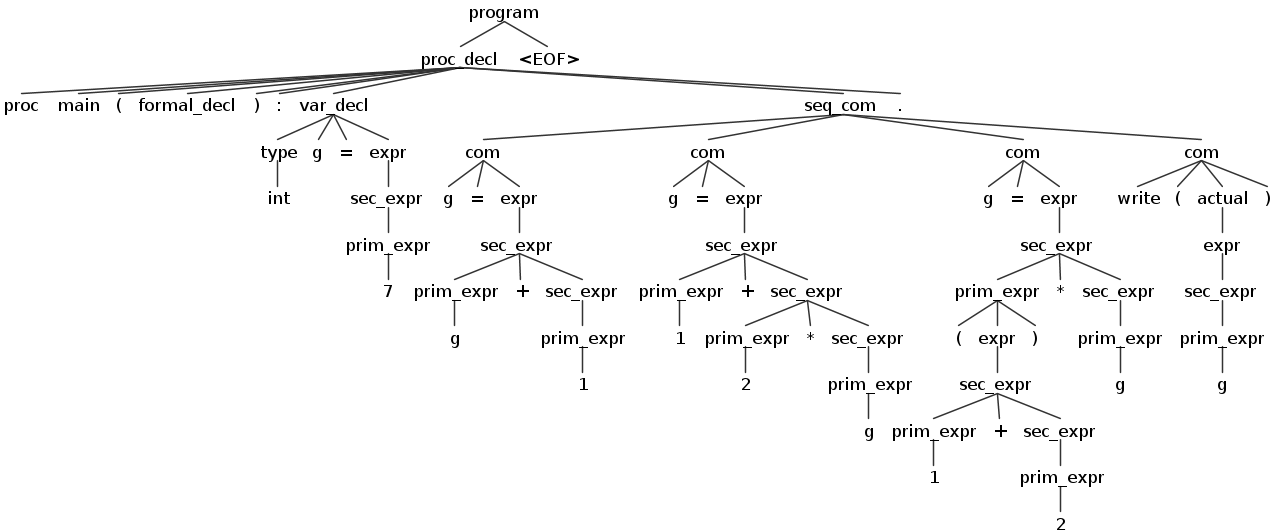
\includegraphics[height=5cm,width=\linewidth]{images/2-2a.png}
		\caption{Parse Tree/Concrete Syntax Tree}
		\label{fig:ANTLR-parse-tree}
	\end{subfigure}
	\begin{subfigure}[b]{0.5\textwidth}
		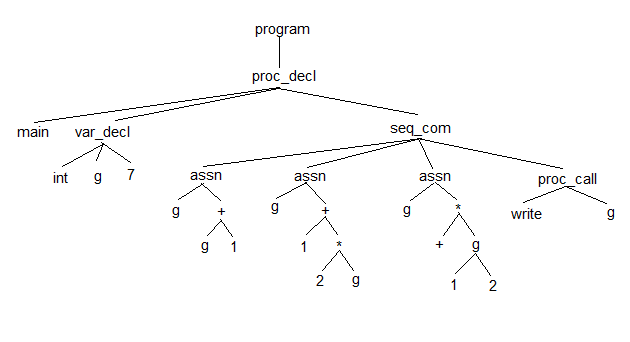
\includegraphics[height=5cm,width=\linewidth]{images/2-2b.png}
		\caption{Abstract Syntax Tree}
		\label{fig:ANTLR-syntax-tree}
	\end{subfigure}
	\caption{The ANTLR generated parse tree and the theoretical AST of the same Fun program}\label{fig:parse-abstract-tree}	
\end{figure}

\chapter{Requirements}
\section{Methodology} 
After establishing that a product is worthwhile to build in the first place, most requirement elicitation approaches involve a repetitive cycle of expanding or reducing an initially small list of desiderata. After an initial interview with Simon Gay, the current lecturer of the {\it Programming Languages} course and proposer of this project, it was clear that whilst the project was inherently complex, the set of functional requirements was simple, well-defined and unlikely to change significantly in the future. For this reason, it was determined that extensive requirement gathering techniques, such as questionnaires or focus groups, were ultimately unnecessary; and all additional requirements were to be established through further interviews with Simon Gay.

\section{User Stories}
User stories are short and simple descriptions of a potential feature, told from the perspective of a potential user. User stories typically follow the template of:\\\\
\textit{As a \textbf{user type}, I want to \textbf{achieve some goal}, so that \textbf{justification.}}

User stories are a core component of the agile software development approach. They provide a means of considering the possible features that various different types of user may want in order to build a fuller set of functional requirements. User stories can also provide the basis for task estimation and prioritisation; however, since this project is not being developed by a team, these aspects won't be considered aside from a high-level prioritisation of end functional requirements.

\begin{itemize}
\item As a user, I want to read details about the Fun language, so that I can write valid Fun programs as input and better understand the compilation animations.
\item As a user, I want to be able to input any Fun program, so that I can learn about the compilation process in the general case, not just for specific examples.
\item As a user, I want to be able to view the animation of the contextual analysis phase of my program, so that I can understand how the compiler carries out this task.
\item As a user, I want to be able to view the animation of the code-generation phase of my program, so that I can understand how the compiler carries out this task.
\item As a user, I want to be able to play different sections of the compilation animation independently (i.e., contextual analysis or code generation), so that I can focus my learning on specific areas. 
\item As a user, I want to be able to replay an animation, so that I can review any details I missed/misunderstood.
\item As a user, I want to be able to step through the animation at my own pace, so I can easier understand what is happening during the animation.
\end{itemize}

\section{Functional Requirements}
After conducting several interviews with Simon Gay and analysing the above user stories, a formal list of functional requirements was created. Functional requirements are intended to capture a specific function of a system. The \textit {MoSCoW method} was used as a prioritisation technique for the following requirements. This method is another commonly used aspect of agile development, and involves partitioning requirements into four categories: \textit{Must have}, \textit{Should have}, \textit{Could have} or \textit{Would have}.
\subsection{Must Have}
\begin{itemize}
\item Allow users to view the AST for pre-defined Fun programs.
\begin{itemize}
\item At the very least, users should be able to choose from a small list of pre-written Fun programs and view the corresponding AST.
\end{itemize}
\end{itemize}
\subsection{Should Have}
\begin{itemize}
\item Allow users to view a simple continuous animation that demonstrates how the AST would be traversed during contextual analysis and code generation.
\begin{itemize}
\item The animation cannot be paused, reversed, or moved through step by step.
\end{itemize}
\item At the end of the animation, display some basic results of the compilation, including object code and address/type tables.
\begin{itemize}
\item These details would only be published at the end of the animation, not during.
\end{itemize}
\item Display information that explains how the Fun language works.
\begin{itemize}
\item This would involve effectively embedding the Fun specification somewhere within the application.
\end{itemize}
\end{itemize}
\subsection{Could Have}
\begin{itemize}
\item Allow users more control over the animation, including pausing, reversing, and step-wise movements - backwards and forwards.
\item Allow users to input any arbitrary Fun program and view the corresponding animation.
\begin{itemize}
\item The user is no longer restricted to using pre-defined example programs.
\end{itemize}
\item Display results of the animation as they occur during the compilation.
\begin{itemize}
\item For example, populate the type table as each variable is declared during the animation.
\end{itemize}
\item Display more in-depth analytical and informational details during the animation.
\begin{itemize}
\item This includes code templates and explanatory messages of the internal workings of each node as it is visited.
\end{itemize}
\end{itemize}
\subsection{Would Have}
\begin{itemize}
\item Execute and display the results of the generated object code.
\end{itemize}

\section{Non-functional Requirements}
In contrast to functional requirements that detail specific behaviours or a system, non-functional requirements measure an overall properties of a system. Non-functional requirements often consider areas such as security, usability and extensibility; overall utilities of a system.

\begin{itemize}
\item The application must work on all modern browsers.
\item The application must be able to interact efficiently with a Java-based application (the Fun compiler).
\item The application must be responsive, at least to a tablet level.
\item The application must ensure no malicious code can be executed.
\end{itemize}

%%%%%%%%%%%%%%%%
%              %
%  APPENDICES  %
%              %
%%%%%%%%%%%%%%%%
\begin{appendices}

\end{appendices}

%%%%%%%%%%%%%%%%%%%%
%   BIBLIOGRAPHY   %
%%%%%%%%%%%%%%%%%%%%

\bibliographystyle{plain}
%\bibliography{bib}

\end{document}
